\documentclass{article}
\usepackage[utf8]{inputenc}

\usepackage{graphicx}
\usepackage{listings}
\usepackage{color}
\usepackage[T1]{fontenc}
\usepackage{lmodern}
\usepackage{textcomp}

\usepackage[top=2cm, bottom=2cm, left=3.5cm, right=3.5cm]{geometry}
 
\definecolor{codegreen}{rgb}{0,0.6,0}
\definecolor{codegray}{rgb}{0.5,0.5,0.5}
\definecolor{codepurple}{rgb}{0.58,0,0.82}
\definecolor{pythonbackcolour}{rgb}{0.95,0.88,0.88}
\definecolor{backcolour}{rgb}{0.88,0.88,0.95}
 
\lstdefinestyle{pythonstyle}{
    language=Python,
    upquote=true,
    backgroundcolor=\color{pythonbackcolour},   
    commentstyle=\color{codegreen},
    keywordstyle=\color{magenta},
    numberstyle=\tiny\color{codegray},
    stringstyle=\color{codepurple},
    basicstyle=\footnotesize\ttfamily,
    basewidth={0.5em,0.5em},
    breakatwhitespace=false,         
    breaklines=true,                 
    captionpos=b,                    
    keepspaces=true,                 
    %numbers=left,                    
    %numbersep=5pt,                  
    showspaces=false,                
    showstringspaces=false,
    showtabs=false,                  
    tabsize=4
}

\lstdefinestyle{bashstyle}{
    language=bash,
    upquote=true,
    backgroundcolor=\color{backcolour},   
    commentstyle=\color{codegreen},
    basicstyle=\footnotesize\ttfamily,
    basewidth={0.5em,0.5em},
    breakatwhitespace=false,         
    breaklines=true,                 
    captionpos=b,                    
    keepspaces=true,                 
    %numbers=left,                    
    %numbersep=5pt,                  
    showspaces=false,                
    showstringspaces=false,
    showtabs=false,                  
    tabsize=4
}
 
\lstset{style=bashstyle}
 
\begin{document}

\title{Getting Started with Auroraplot}
%\date{}
\maketitle

\section{Minimum Requirements}

Auroraplot has been tested on Ubuntu 16.04 LTS and Debian 8.
It should work on other linux distributions and Apple's MacOS with minimal changes to the installation and configuration steps. Microsoft Windows is not currently supported.

Loading and manipulating large data sets requires a significant amount of RAM.
On systems with 8 GB frequent swapping to disk and slow-downs can occur,
especially when creating Quiet Day Curves. 16 GB is recommended.

\section{Installation}
\label{install}

First install the dependencies. In a terminal type

\begin{figure}[htb!]
\begin{minipage}[b]{0.45\linewidth}
Fedora 25
\begin{lstlisting}
sudo dnf upgrade
sudo dnf install python-pyside git python2-matplotlib-qt4 python-requests python-ipython python-scipy python-pandas
\end{lstlisting}
\end{minipage}
\hspace{0.5cm}
\begin{minipage}[b]{0.45\linewidth}
Ubuntu 16.04 LTS / Debian 8
\begin{lstlisting}
sudo apt update
sudo apt upgrade                 
sudo apt install git ipython python-matplotlib python-scipy python-pyside python-requests python-pandas 
\end{lstlisting}
\end{minipage} 
\end{figure}

\noindent {\bf python-pandas} is an optional dependency (54.8 MB) that will speed up the loading of data.

%\subsection{Installing the latest version of Auroraplot}
To install Auroraplot in your home folder type
\begin{lstlisting}
cd ~
git clone https://github.com/m-j-b/auroraplot.git
\end{lstlisting}

Python looks in the in the {\it site-packages} folder for installed python packages. Create the {\it site-packages} folder, and in it create a symlink to the Auroraplot package.

\begin{lstlisting}
mkdir -p ~/.local/lib/python2.7/site-packages
ln -s ~/auroraplot/auroraplot ~/.local/lib/python2.7/site-packages/
\end{lstlisting}

Compile Auroraplot binaries for your system

\begin{lstlisting}
make -C ~/auroraplot/
\end{lstlisting}

Make a desktop launcher for the Auroraplot GUI.
\begin{lstlisting}
mkdir -p ~/.local/share/applications/
ln -s ~/.local/lib/python2.7/site-packages/auroraplot/gui/auroraplotx.desktop ~/.local/share/applications/
xdg-icon-resource install --novendor --size 128 ~/.local/lib/python2.7/site-packages/auroraplot/gui/icons/auroraplot_128.png
\end{lstlisting}

Once Auroraplot is installed it can be updated to the latest version by running
\begin{lstlisting}
cd ~/auroraplot/
git fetch --all
git checkout --force master
make -C ~/auroraplot/ clean
make -C ~/auroraplot/
\end{lstlisting}


\section{Using Auroraplot in IPython}

IPython is a convenient command line interface for python, it includes command history, tab-completion, etc.
By default, scripts that are imported into python and subsequently edited will not be automatically reloaded. To change this behaviour, create a startup file for IPython.

\begin{lstlisting}
mkdir -p ~/.ipython/profile_default/startup/
nano ~/.ipython/profile_default/startup/10-custom.ipy
\end{lstlisting}

In the file enter (including the \% symbols)
\begin{lstlisting}[style=pythonstyle]
%load_ext autoreload
%autoreload 2
%pylab
\end{lstlisting}

\subsection{IPython Examples}

To speed up loading of data, copy the example riometer data (1.5 GB) to the /data directory, which is the default data location in Auroraplot.

\begin{lstlisting}
sudo mkdir /data
sudo wget -m -np -nH --cut-dirs 1 -P /data -A *.txt http://www.riometer.net/example_data/2004
\end{lstlisting}

Create a directory for Quiet Day Curves (QDCs), and a group ({\it qdc}) for users that have permission to create and modify QDCs in that directory.

\begin{lstlisting}
sudo groupadd qdc
sudo mkdir /data/qdc
sudo chown root:qdc /data/qdc
sudo chmod g+w /data/qdc
\end{lstlisting}

If required, add the current user to the {\it qdc} group. (The user will need to log out and back in for this to take effect).

\begin{lstlisting}
sudo usermod -aG qdc $USER
\end{lstlisting}

Begin an IPython session with the command

\begin{lstlisting}
ipython
\end{lstlisting}

It is helpful to see the logger output in IPython. This will indicate errors and failures to load data. To have log messages display on the screen run

\begin{lstlisting}[style=pythonstyle]
import logging
logging.basicConfig(stream=sys.stdout, level=logging.DEBUG)
\end{lstlisting}

For each one of these examples, you will first need to import Auroraplot and the datasets into IPython.

\begin{lstlisting}[style=pythonstyle]
# import the riodata module, and the datasets metadata
import auroraplot as ap
import auroraplot.riodata as riodata
import auroraplot.datasets.riometernet
\end{lstlisting}


\subsubsection{Example 1: Plotting Riometer Power Data}

In this example, we load one day of riometer power data from beam 25 of the Kilpisj\"arvi riometer, KIL1 (also known as IRIS). The example data covers January 2004, but we will load and plot data from 22 January 2004.

\begin{lstlisting}[style=pythonstyle]
# set the start and end times
st = np.datetime64('2004-01-22T00:00:00')
et = st + np.timedelta64(1,'D')

# load the power data
rd = ap.load_data('RN','KIL1','RioPower',st,et,'local archive',['25'])

# plot the data
rd.plot()
\end{lstlisting}

\begin{center}
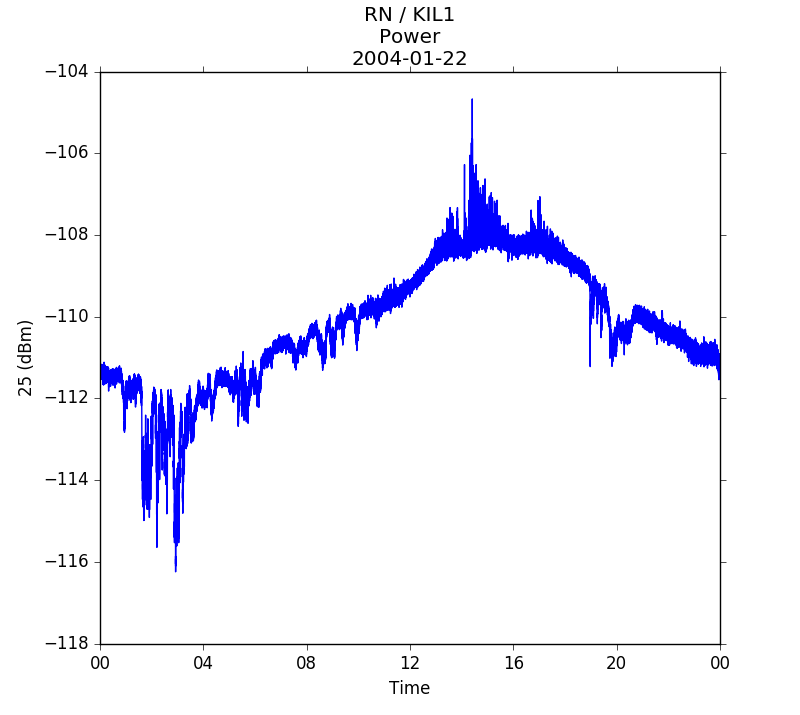
\includegraphics[width=9cm]{images/figure_1.png}
\end{center}

\noindent Hints on how to use functions such as {\bf ap.load\_data} can be seen by appending a question mark to the function name.

\begin{lstlisting}[style=pythonstyle]
ap.load_data?

Definition:  ap.load_data(project, site, data_type, start_time, end_time, archive=None, channels=None, path=None, load_function=None, raise_all=False, cadence=None, aggregate=None, filter_function=None)
\end{lstlisting}

Each riometer has a site name (in this case 'KIL1'), and belongs to a particular project. 'RN' stands for the Riometer Network project. The archive name 'local archive' could be changed to 'remote archive' in order to load this example data from www.riometer.net. Sites, projects and archives are defined in the datasets module ({\bf auroraplot.datasets.riometernet}).

Note that the channels are specified as a list of strings. When dealing with riometer data, channels (beams) are usually numbered from 1, but magnetometer channels may be named 'X', 'Y', and 'Z', or 'H', 'D', and 'Z'.


\subsubsection{Example 2: Quiet Day Curves and Ionospheric Absorption}

To make a quiet day curve it is necessary to load more than one day of data. Usually 14 days will suffice. By default, the valid period for a QDC will be 14 days long.
Auroraplot has functions in the {\bf ap.dt64tools} package that can be used to find the standard boundaries for the QDCs: {\bf ap.dt64tools.floor}, and {\bf ap.dt64tools.ceil}. If the period is a multiple of one week, the boundary will begin on a Monday.

\begin{lstlisting}[style=pythonstyle]
t = np.datetime64('2004-01-22T00:00:00')
st = ap.dt64tools.floor(t, np.timedelta64(14,'D'))
et = ap.dt64tools.ceil(t, np.timedelta64(14,'D'))
rd = ap.load_data('RN','KIL1','RioPower',st,et,'local archive',channels=['25'])
\end{lstlisting}

\noindent Here {\it st} holds the {\bf numpy.datetime64} value of '2004-01-12T00:00:00', and {\it et} is '2004-01-26T00:00:00'.

The QDC is made from the power data by calling {\bf make\_qdc()}.

\begin{lstlisting}[style=pythonstyle]
qdc = rd.make_qdc()
qdc.plot(channels=['25'])
\end{lstlisting}

\begin{center}
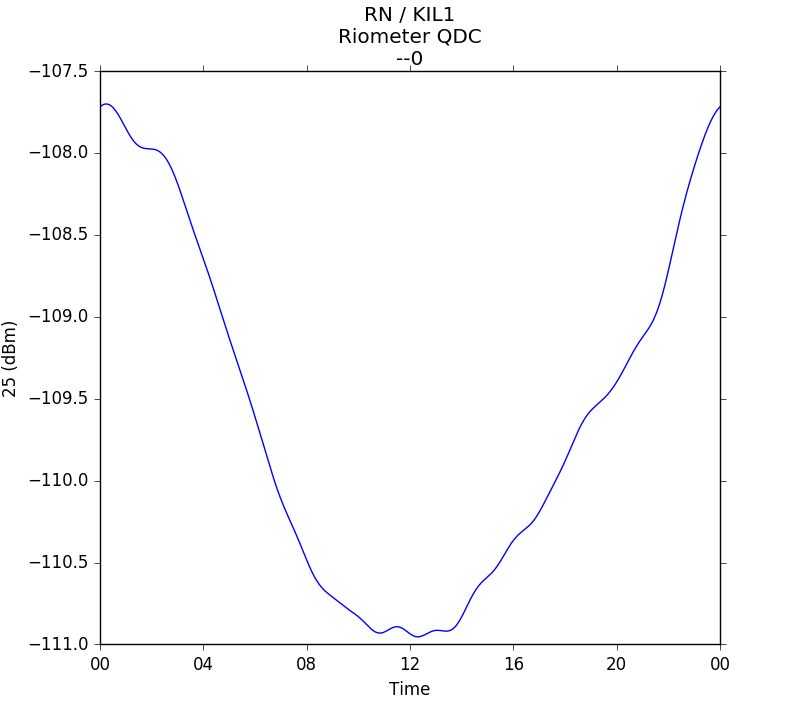
\includegraphics[width=9cm]{images/figure_2.png}
\end{center}


\noindent Calling {\bf make\_qdc()} will create QDCs for all channels of the riometer (according to the metadata in auroraplot.datasets). But since {\it rd} only contains data for channel 25, calling {\bf qdc.plot()}, without the {\it channels} argument would make a large number of mostly empty plots.

If the computer has sufficient RAM ($\ge 12$ GB recommended) data from all channels can be loaded at once. It is advantageous to integrate the riometer to lower resolutions before creating the quiet day curve.

\begin{lstlisting}[style=pythonstyle]
rd = ap.load_data('RN','KIL1','RioPower',st,et,'local archive')
rd.set_cadence(np.timedelta64(10,'s'), inplace=True)
qdc = rd.make_qdc()
qdc.plot(channels=['24','25','31','32'])
\end{lstlisting}

\begin{center}
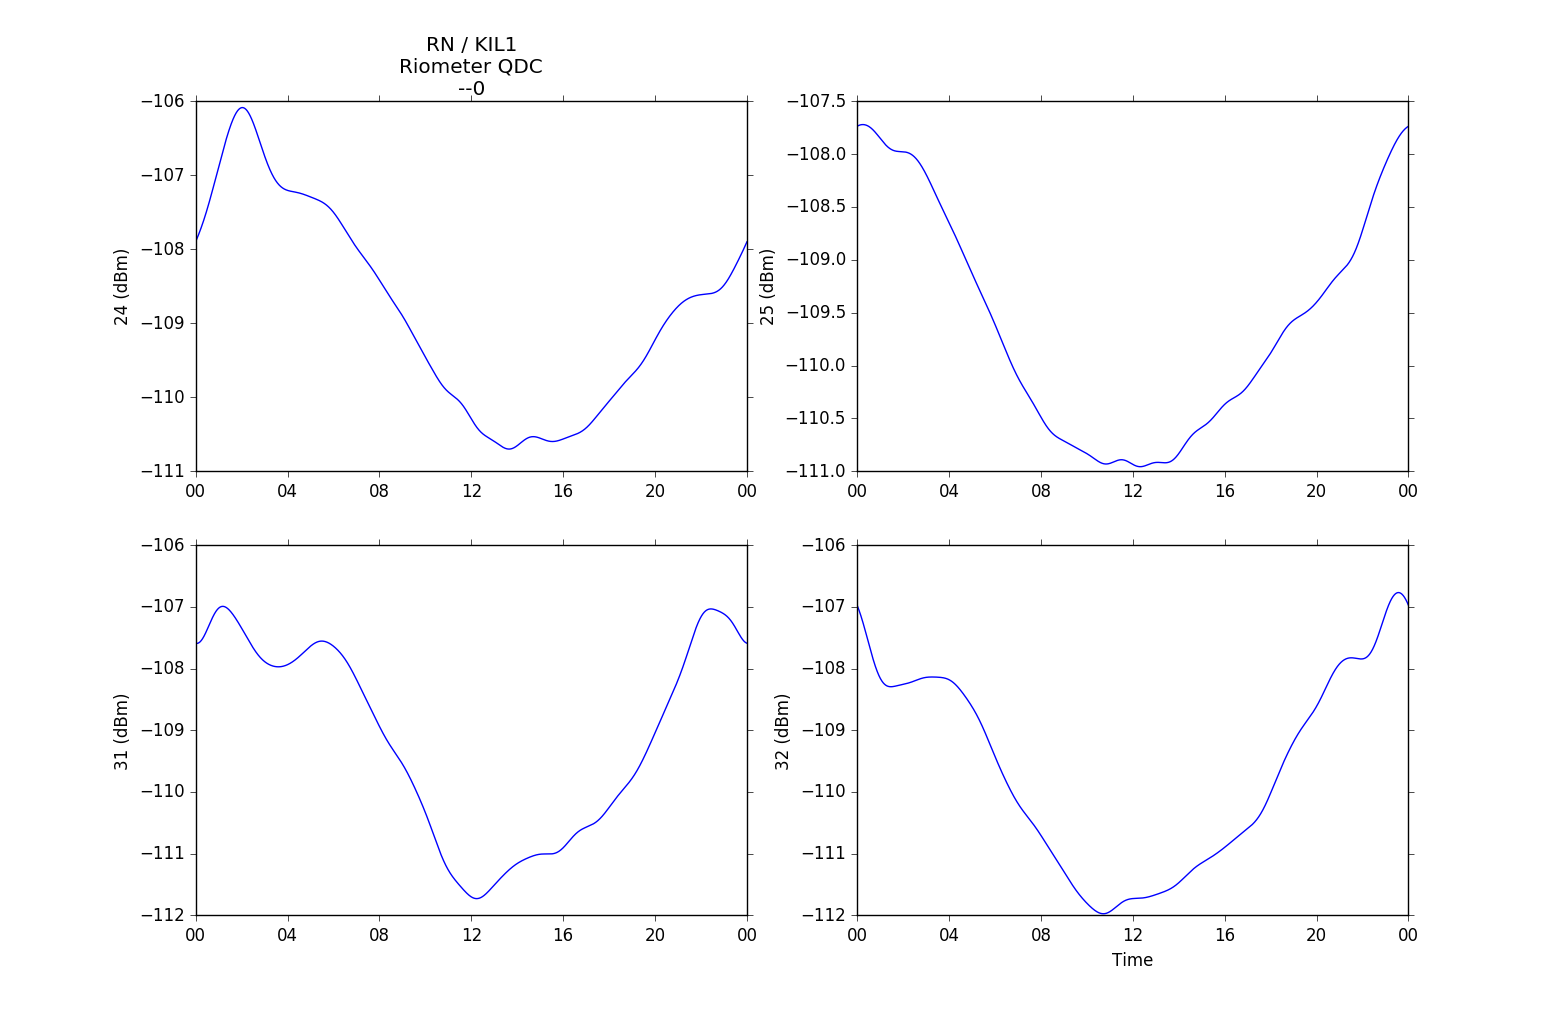
\includegraphics[width=13cm]{images/figure_3.png}
\end{center}

\noindent The argument {\it inplace=True} tells {\bf set\_cadence} to overwrite {\it rd} instead of returning a copy of it with the new cadence (sampling interval).

The QDC can be saved for later use.

\begin{lstlisting}[style=pythonstyle]
qdc.save(archive='local archive', time=t)
\end{lstlisting}

\noindent {\it time} is any {\bf numpy.datetime64} within the QDC's valid period. This will save the QDC to /data/qdc/kil1/2004/kil1\_qdc\_20040112.txt.

The QDC can be reloaded by specifying the project, site, and a time within its valid period.

\begin{lstlisting}[style=pythonstyle]
qdc = ap.riodata.load_qdc('RN', 'KIL1', t, archive='local archive')
\end{lstlisting}

We can look again at the data from 22 January 2004, and this time plot it alongside the QDC.

\begin{lstlisting}[style=pythonstyle]
st = np.datetime64('2004-01-22T00:00:00')
et = st + np.timedelta64(1,'D')
rd = ap.load_data('RN','KIL1','RioPower',st,et,'local archive',channels=['25'])
rd.plot_with_qdc(qdc)
\end{lstlisting}

\begin{center}
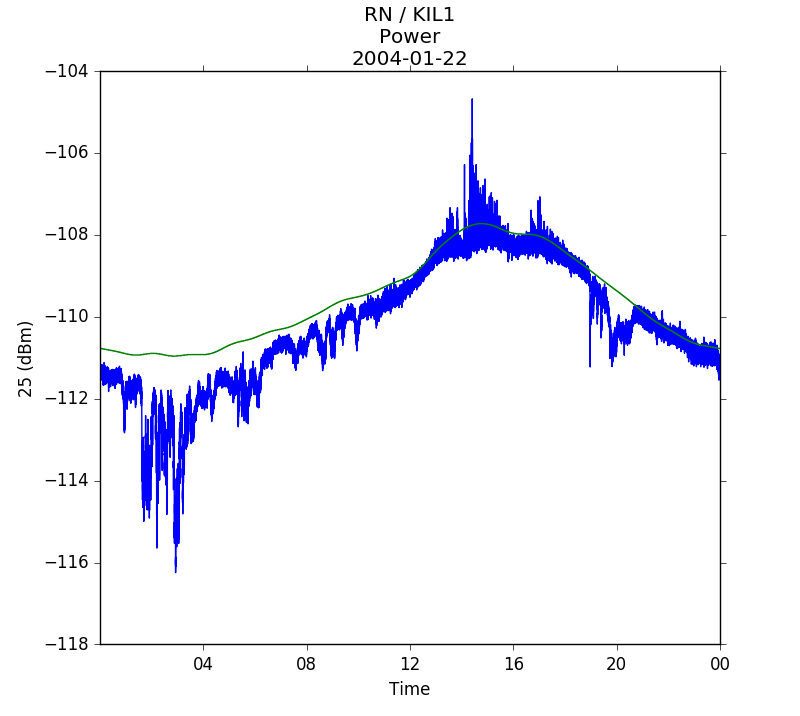
\includegraphics[width=9cm]{images/figure_4.png}
\end{center}


\noindent Alternatively, we can plot the ionospheric absorption (i.e. the quiet day curve minus the riometer received power).
\begin{lstlisting}[style=pythonstyle]
ab = rd.apply_qdc(qdc)
ab.plot()
\end{lstlisting}

\begin{center}
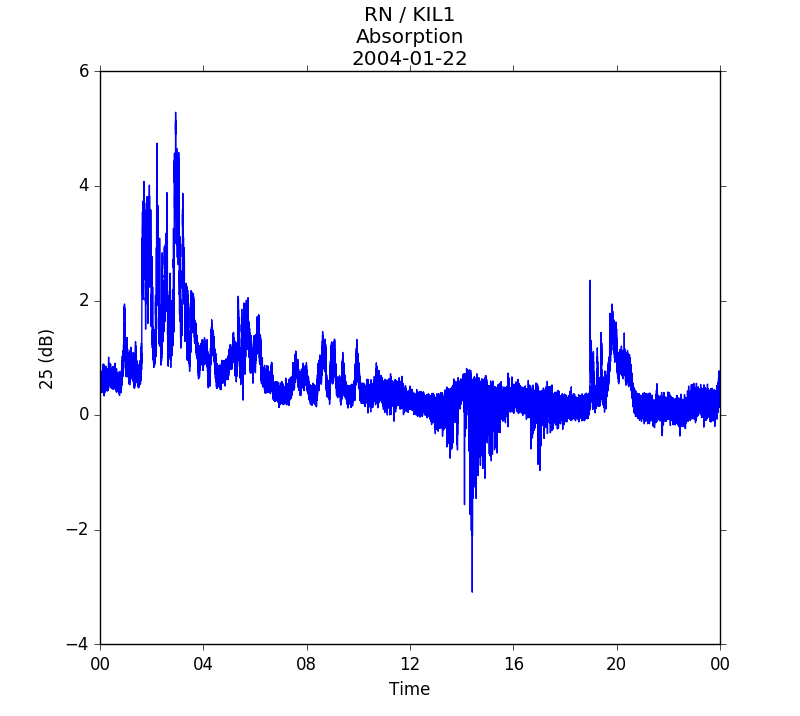
\includegraphics[width=9cm]{images/figure_5.png}
\end{center}

\subsubsection{Example 3: Integration and Further Processing}

In this example, we calculate the ionospheric absorption for the 21st, 22nd and 23rd of January, beams 25 and 26. Then integrate the data to 6 hour resolution, plot it, and extract the data of beam 25 for further processing. We will use the QDC saved in the previous example.

\begin{lstlisting}[style=pythonstyle]
st = np.datetime64('2004-01-21T00:00:00')
et = st + np.timedelta64(3,'D')
rd = ap.load_data('RN','KIL1','RioPower',st,et,'local archive',channels=['25','26'])
qdc = ap.riodata.load_qdc('RN', 'KIL1', st, archive='local archive')
ad = rd.apply_qdc(qdc)
ad6hr = ad.set_cadence(np.timedelta64(6,'h'))
ad6hr.plot(step_plot=True)
\end{lstlisting}

\begin{center}
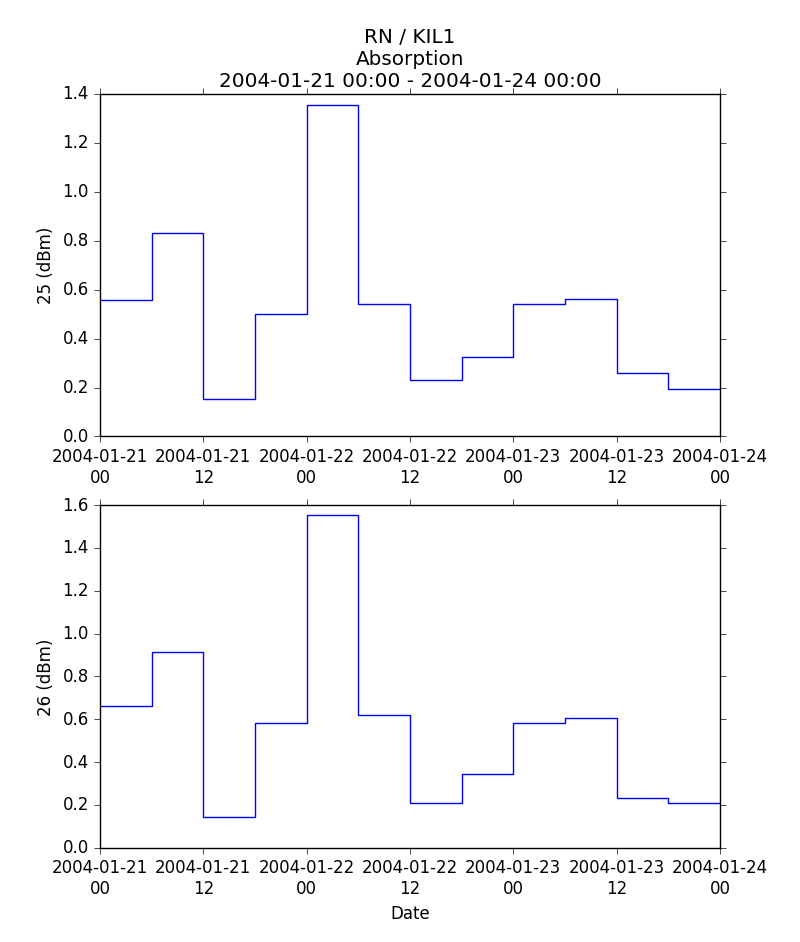
\includegraphics[width=9cm]{images/figure_6.png}
\end{center}

\noindent Note how the absorption tends to be higher in the early hours of each morning. This is a common feature since the morning sector is strongly affected by electron precipitation following substorms.
 
To extract the data for beam 25, and find the central time of each sample.

\begin{lstlisting}[style=pythonstyle]
b25_index = ad6hr.get_channel_index(['25'])
b25_absorption_data = ad6hr.data[b25_index]
sample_central_time = ap.dt64tools.mean(ad6hr.sample_start_time,ad6hr.sample_end_time) 
\end{lstlisting}

\newpage 

\section{The Quick-Look Data Viewer}

\begin{center}
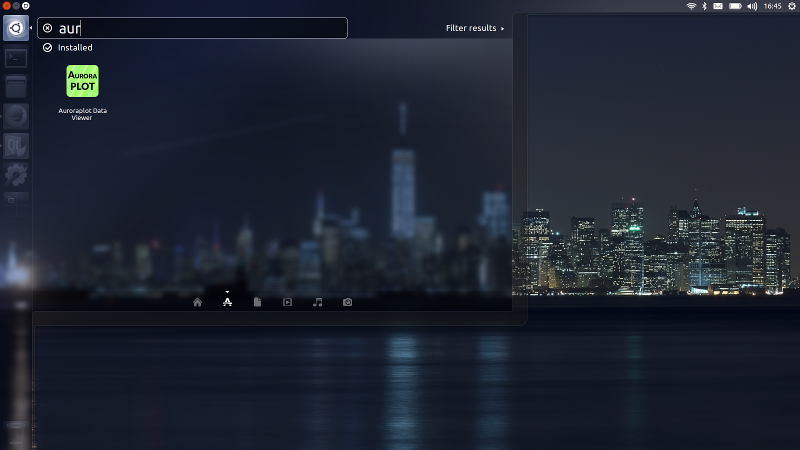
\includegraphics[width=15cm]{images/dv-0.png}
\end{center}

If you followed the instructions in section \ref{install}, a desktop launcher for the Auroraplot GUI should already be on your system.

The following tour of the data viewer assumes that you have completed the previous sections and saved the quiet day curves for the example data. If not, you will be able to load the data from a remote archive, but this is much slower.

\begin{center}
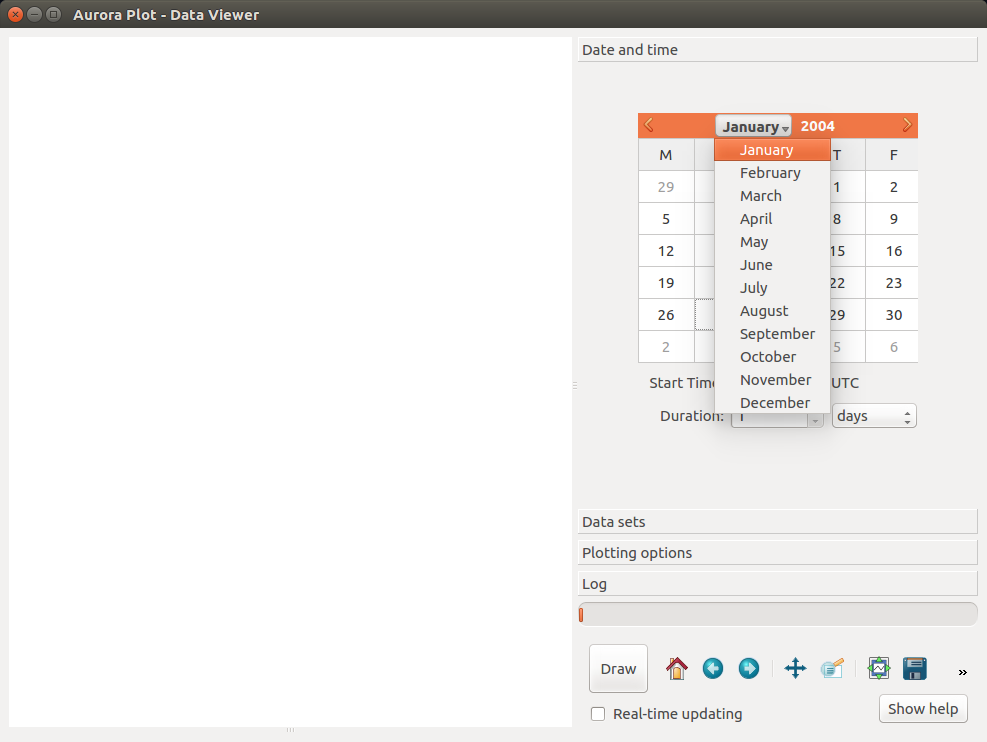
\includegraphics[width=11cm]{images/dv-1.png}
\end{center}

Select a start time and date in January 2004 -- the month covered by the example data. You can select any reasonable duration for the plots.
Be sure to click on the start date in the calendar. Then click on the {\it Data sets} tab to choose some data to plot.

\begin{center}
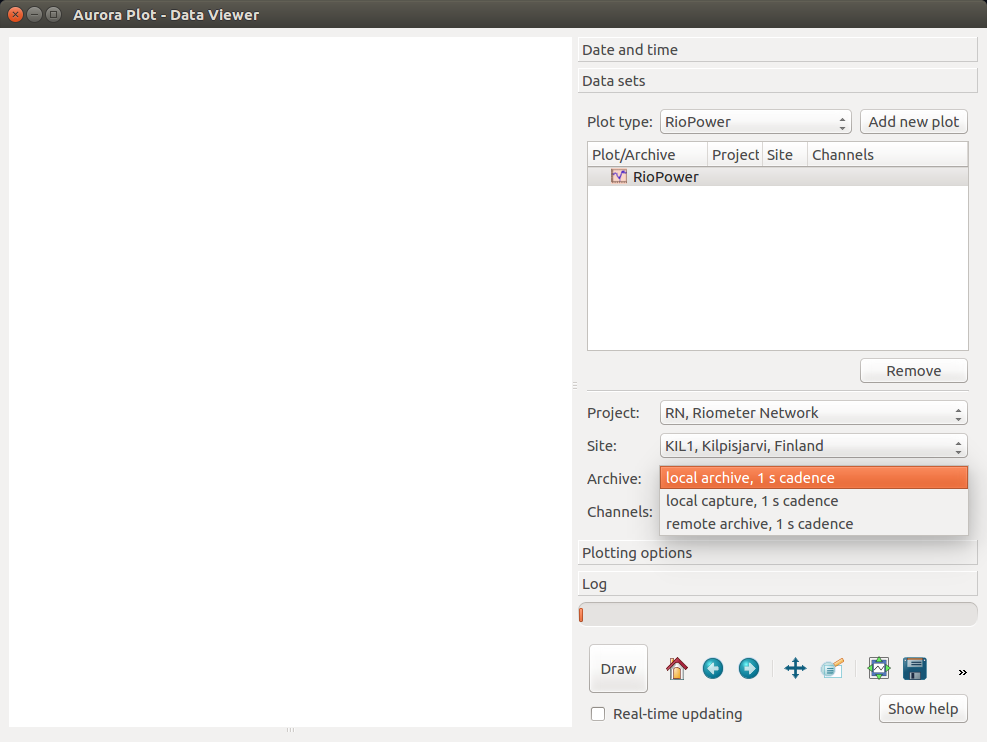
\includegraphics[width=11cm]{images/dv-2.png}
\end{center}

\noindent In the {\it Data sets} tab, choose {\bf RioPower} (riometer power) for the data type. {\bf RioPower} is also used for plotting ionospheric absorption, because the absorption is calculated from the power received by the riometer.

Click {\bf Add new plot} to add the new {\bf RioPower} plot to the list.
If you make a mistake, you can remove items from the list by selecting them and clicking {\bf Remove}.

Next add the KIL1 data to the plot. Select {\bf local archive} if you have completed the examples in the previous sections. Otherwise you can use the (much slower) {\bf remote archive}.

Enter the channels (beams) to add to the plot, seperated by commas. For the first plot, we chose 17, 18, 19. Then click {\bf Add data set} to add the data set to the selected plot in the list.

\begin{center}
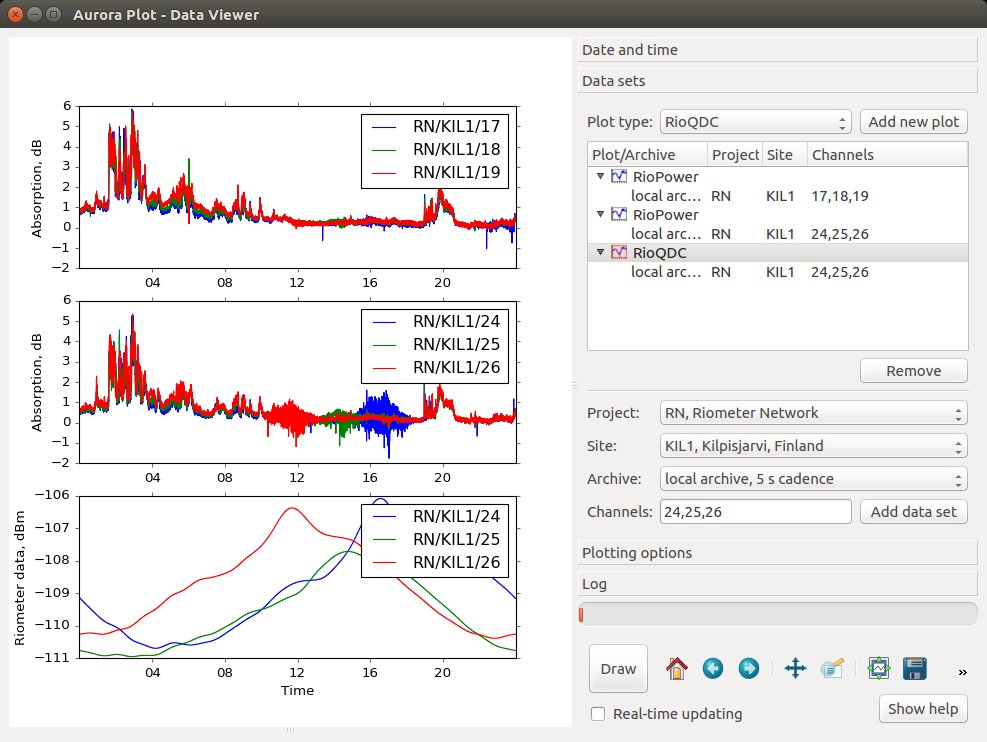
\includegraphics[width=11cm]{images/dv-3.png}
\end{center}

Here 3 plots, and 3 data sets have been added to the list. The last plot is of the {\bf RioQDC} type. Click {\bf Draw} to load the data and make the plots.

In the middle plot there is ionospheric scintillation. It looks like noise, and it is first seen in beam 26 at midday, then 25, then 24. 
It moves from beam to beam as the source of the scintillation progresses through the riometer array as Earth rotates.

\begin{center}
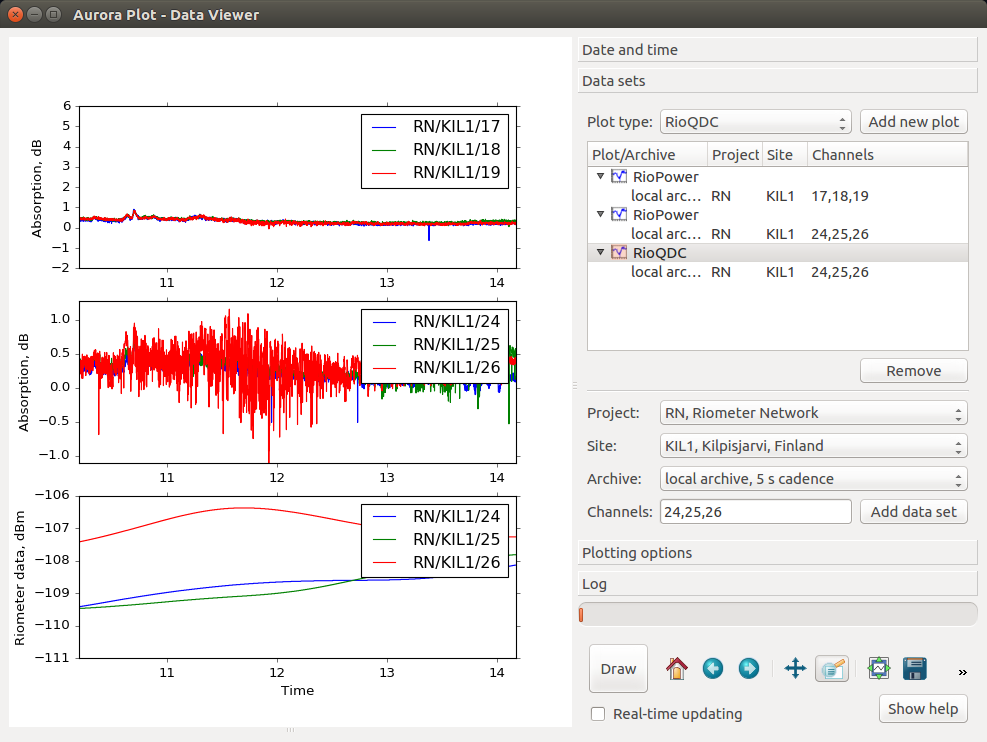
\includegraphics[width=11cm]{images/dv-4.png}
\end{center}

The buttons to the right of {\bf Draw} are tools to change the view, and save the plots as an image file. Here we have zoomed in on the scintillation in beam 26.

\begin{center}
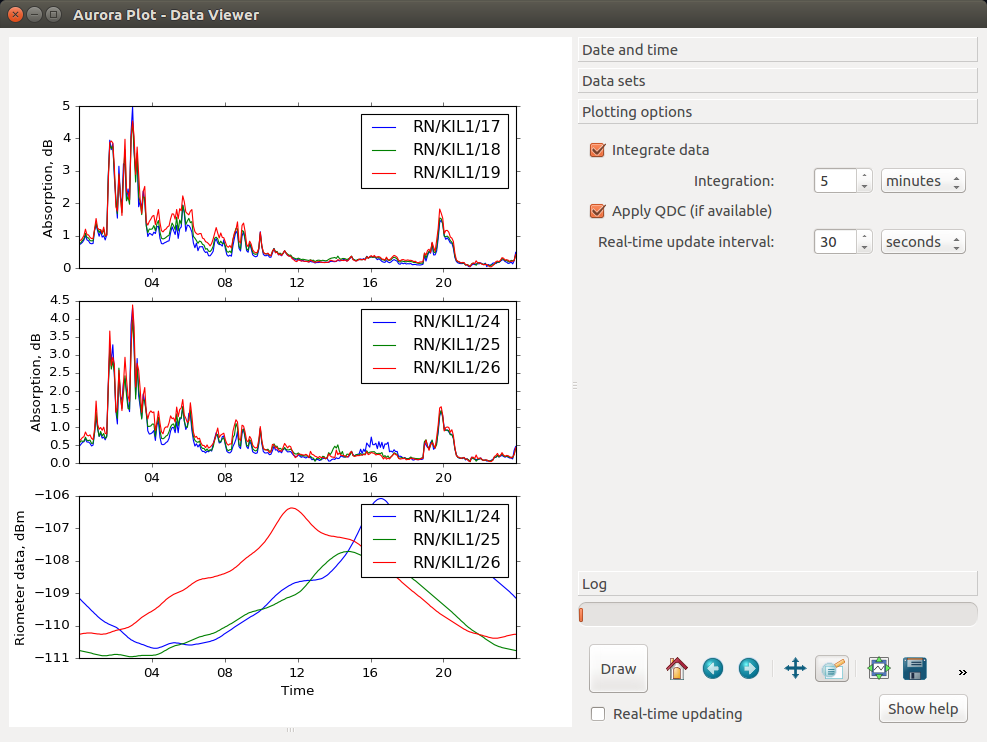
\includegraphics[width=11cm]{images/dv-5.png}
\end{center}

To reduce noise and scintillation in the data it is possible to perform integration. Click on the {\it Plotting options} tab.

\begin{center}
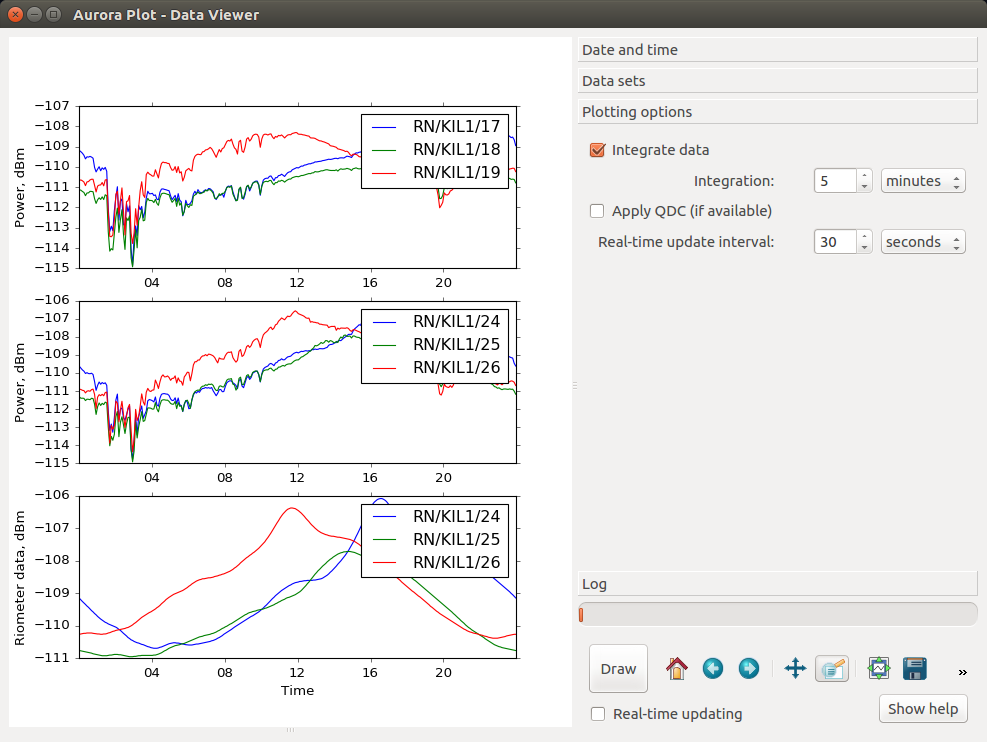
\includegraphics[width=11cm]{images/dv-6.png}
\end{center}

\noindent In the plotting options change the integration from 5 seconds to 5 minutes. This is more than enough to smooth the scintillation. Click {\bf Draw} to redraw the plots.

\begin{center}
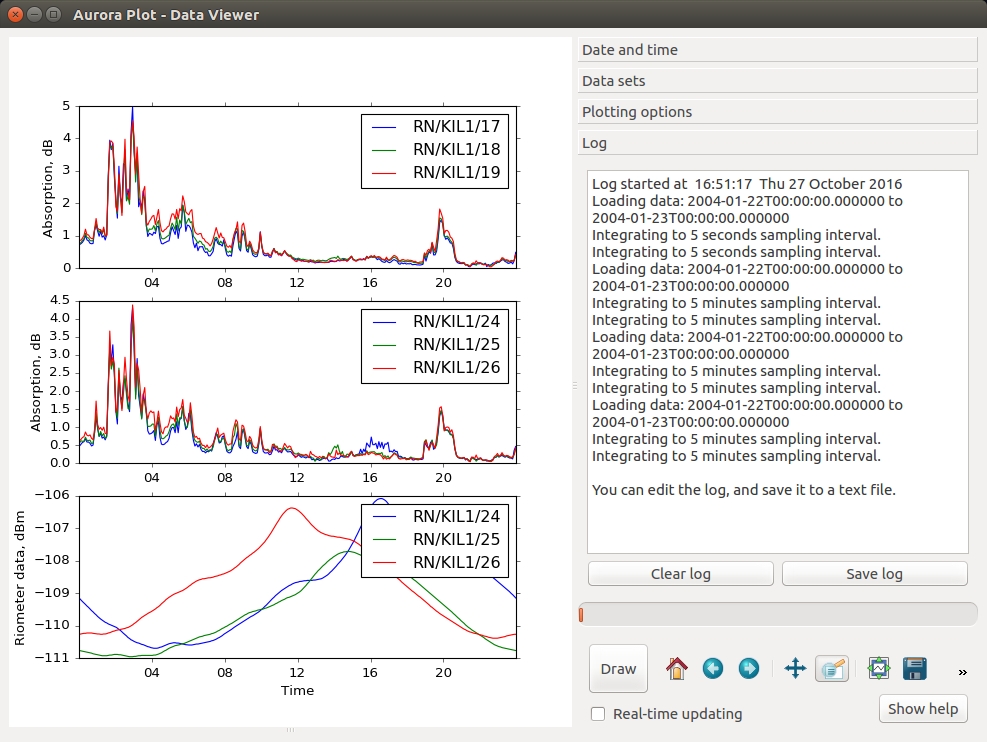
\includegraphics[width=11cm]{images/dv-7.png}
\end{center}

Finally the {\it Logging} tab shows a log of what is being plotted and when, and describes any errors that might occur. It is possible to edit the log by typing into the window, and to save it to a text file.


\end{document}

